% Options for packages loaded elsewhere
\PassOptionsToPackage{unicode}{hyperref}
\PassOptionsToPackage{hyphens}{url}
%
\documentclass[
]{article}
\usepackage{lmodern}
\usepackage{amssymb,amsmath}
\usepackage{ifxetex,ifluatex}
\ifnum 0\ifxetex 1\fi\ifluatex 1\fi=0 % if pdftex
  \usepackage[T1]{fontenc}
  \usepackage[utf8]{inputenc}
  \usepackage{textcomp} % provide euro and other symbols
\else % if luatex or xetex
  \usepackage{unicode-math}
  \defaultfontfeatures{Scale=MatchLowercase}
  \defaultfontfeatures[\rmfamily]{Ligatures=TeX,Scale=1}
\fi
% Use upquote if available, for straight quotes in verbatim environments
\IfFileExists{upquote.sty}{\usepackage{upquote}}{}
\IfFileExists{microtype.sty}{% use microtype if available
  \usepackage[]{microtype}
  \UseMicrotypeSet[protrusion]{basicmath} % disable protrusion for tt fonts
}{}
\makeatletter
\@ifundefined{KOMAClassName}{% if non-KOMA class
  \IfFileExists{parskip.sty}{%
    \usepackage{parskip}
  }{% else
    \setlength{\parindent}{0pt}
    \setlength{\parskip}{6pt plus 2pt minus 1pt}}
}{% if KOMA class
  \KOMAoptions{parskip=half}}
\makeatother
\usepackage{xcolor}
\IfFileExists{xurl.sty}{\usepackage{xurl}}{} % add URL line breaks if available
\IfFileExists{bookmark.sty}{\usepackage{bookmark}}{\usepackage{hyperref}}
\hypersetup{
  pdftitle={Assignment 04},
  pdfauthor={Nosky, Christopher},
  hidelinks,
  pdfcreator={LaTeX via pandoc}}
\urlstyle{same} % disable monospaced font for URLs
\usepackage[margin=1in]{geometry}
\usepackage{longtable,booktabs}
% Correct order of tables after \paragraph or \subparagraph
\usepackage{etoolbox}
\makeatletter
\patchcmd\longtable{\par}{\if@noskipsec\mbox{}\fi\par}{}{}
\makeatother
% Allow footnotes in longtable head/foot
\IfFileExists{footnotehyper.sty}{\usepackage{footnotehyper}}{\usepackage{footnote}}
\makesavenoteenv{longtable}
\usepackage{graphicx,grffile}
\makeatletter
\def\maxwidth{\ifdim\Gin@nat@width>\linewidth\linewidth\else\Gin@nat@width\fi}
\def\maxheight{\ifdim\Gin@nat@height>\textheight\textheight\else\Gin@nat@height\fi}
\makeatother
% Scale images if necessary, so that they will not overflow the page
% margins by default, and it is still possible to overwrite the defaults
% using explicit options in \includegraphics[width, height, ...]{}
\setkeys{Gin}{width=\maxwidth,height=\maxheight,keepaspectratio}
% Set default figure placement to htbp
\makeatletter
\def\fps@figure{htbp}
\makeatother
\setlength{\emergencystretch}{3em} % prevent overfull lines
\providecommand{\tightlist}{%
  \setlength{\itemsep}{0pt}\setlength{\parskip}{0pt}}
\setcounter{secnumdepth}{-\maxdimen} % remove section numbering

\title{Assignment 04}
\author{Nosky, Christopher}
\date{1/10/2021}

\begin{document}
\maketitle

\hypertarget{markdown-basics}{%
\section{Markdown Basics}\label{markdown-basics}}

\hypertarget{favorite-foods}{%
\subsection{Favorite Foods}\label{favorite-foods}}

\begin{enumerate}
\def\labelenumi{\arabic{enumi}.}
\tightlist
\item
  Brisket
\item
  Pizza
\item
  Bacon
\end{enumerate}

\hypertarget{images}{%
\subsection{Images}\label{images}}

\begin{figure}
\centering
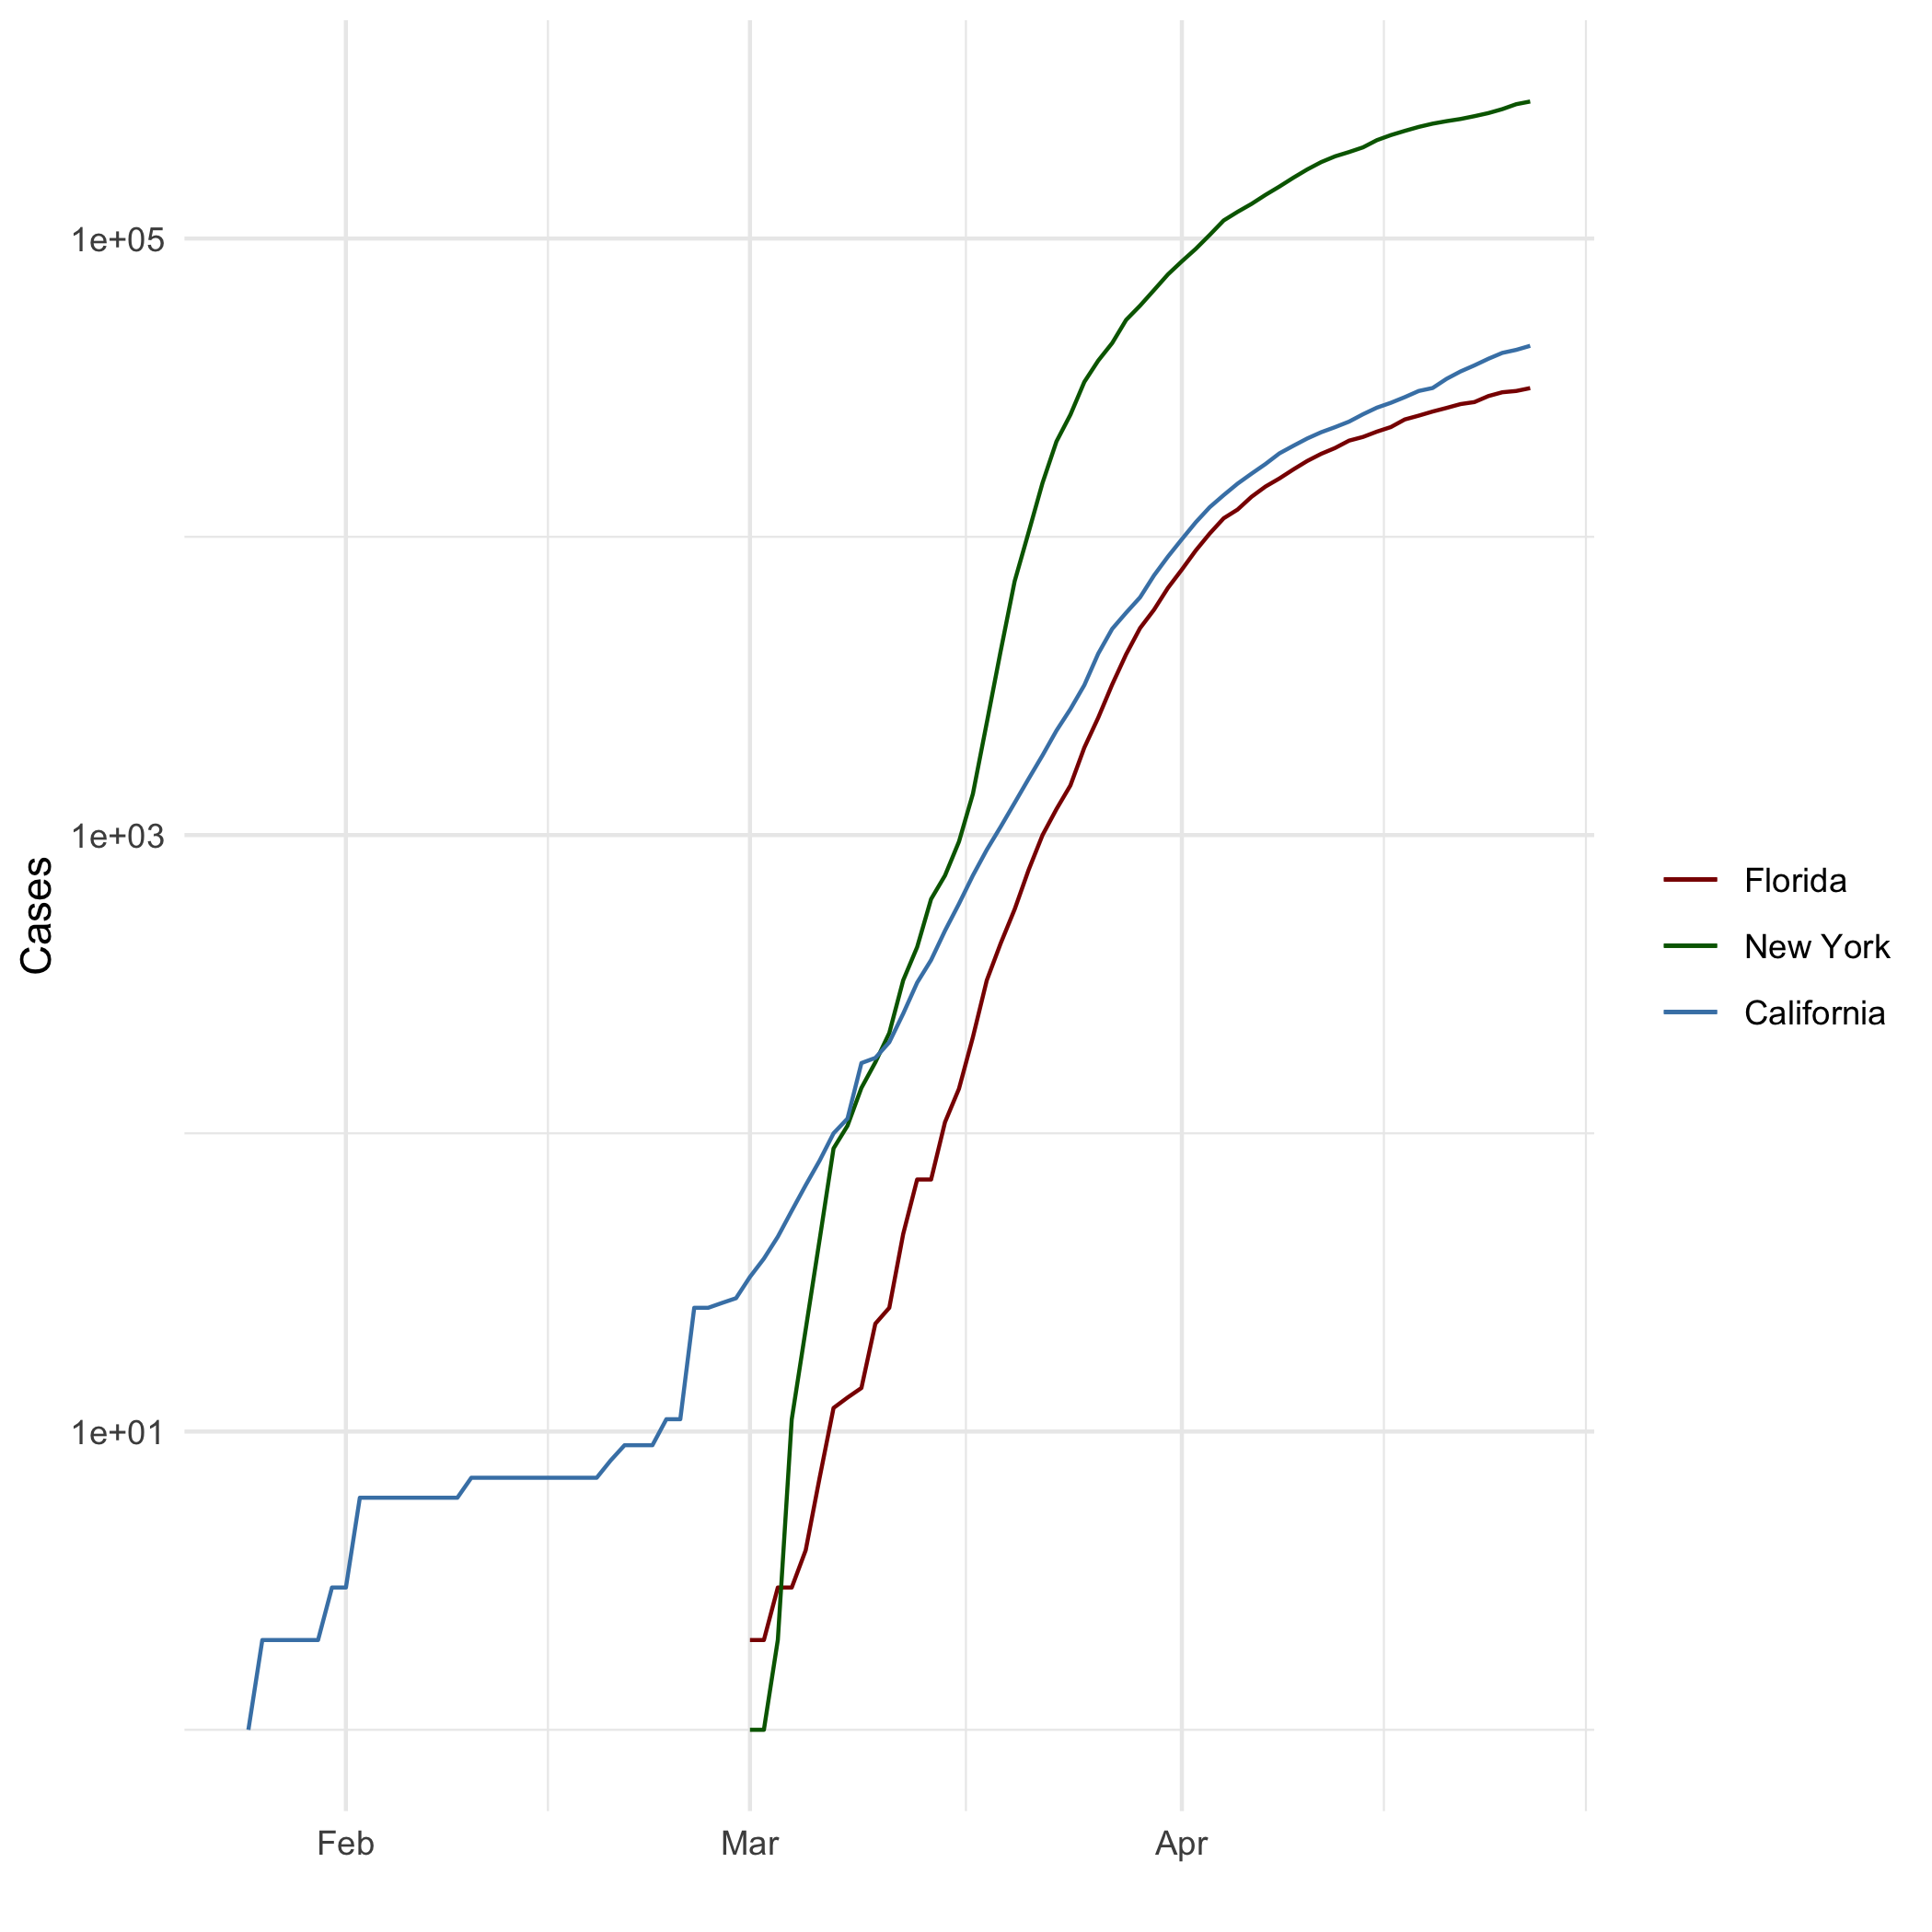
\includegraphics{C:/Users/cwnos/Documents/DSC520/Git repo/DSC520/dsc520/completed/assignment04/plots/10-all-cases-log.png}
\caption{All Cases (Log Plot)}
\end{figure}

\hypertarget{add-a-quote}{%
\subsection{Add a Quote}\label{add-a-quote}}

\hypertarget{be-yourself-everyone-else-is-already-taken.-oscar-wilde}{%
\subsubsection{\texorpdfstring{\emph{``Be yourself; everyone else is
already taken.''} \emph{Oscar
Wilde}}{``Be yourself; everyone else is already taken.'' Oscar Wilde}}\label{be-yourself-everyone-else-is-already-taken.-oscar-wilde}}

\hypertarget{add-an-equation}{%
\subsection{Add an Equation}\label{add-an-equation}}

\hypertarget{emc2}{%
\subparagraph{\texorpdfstring{\(E=mc^2\)}{E=mc\^{}2}}\label{emc2}}

\hypertarget{add-a-footnote}{%
\subsection{Add a Footnote}\label{add-a-footnote}}

A footnote you say?,\footnote{Where would I get an idea like that.} and
since I didn't know which is preferred.\footnote{Both examples of a
  footnote, choose which works best for you.

  You can also indent paragraphs and code to include them in the
  footnote.

  \texttt{\{\ my\ code\ \}}

  Add as many paragraphs as you like.}

\hypertarget{add-citations}{%
\subsection{Add Citations}\label{add-citations}}

\begin{itemize}
\tightlist
\item
  R for Everyone (see Lander 2014)
\item
  Discovering Statistics Using R (see Field, Miles, and Field 2012)
\end{itemize}

\hypertarget{inline-code}{%
\section{Inline Code}\label{inline-code}}

\hypertarget{ny-times-covid-19-data}{%
\subsection{NY Times COVID-19 Data}\label{ny-times-covid-19-data}}

\begin{verbatim}
## Warning: package 'ggplot2' was built under R version 4.0.3
\end{verbatim}

\includegraphics{Exercise_07_NoskyChristopher_files/figure-latex/ggplot-a-1.pdf}

\hypertarget{r4ds-height-vs-earnings}{%
\subsection{R4DS Height vs Earnings}\label{r4ds-height-vs-earnings}}

\includegraphics{Exercise_07_NoskyChristopher_files/figure-latex/ggplot-b-1.pdf}

\hypertarget{tables}{%
\section{Tables}\label{tables}}

\hypertarget{knitr-table-with-kable}{%
\subsection{Knitr Table with Kable}\label{knitr-table-with-kable}}

\begin{longtable}[]{@{}llllr@{}}
\caption{One Ring to Rule Them All}\tabularnewline
\toprule
name & race & in\_fellowship & ring\_bearer & age\tabularnewline
\midrule
\endfirsthead
\toprule
name & race & in\_fellowship & ring\_bearer & age\tabularnewline
\midrule
\endhead
Aragon & Men & TRUE & FALSE & 88\tabularnewline
Bilbo & Hobbit & FALSE & TRUE & 129\tabularnewline
Frodo & Hobbit & TRUE & TRUE & 51\tabularnewline
Galadriel & Elf & FALSE & FALSE & 7000\tabularnewline
Sam & Hobbit & TRUE & TRUE & 36\tabularnewline
Gandalf & Maia & TRUE & TRUE & 2019\tabularnewline
Legolas & Elf & TRUE & FALSE & 2931\tabularnewline
Sauron & Maia & FALSE & TRUE & 7052\tabularnewline
Gollum & Hobbit & FALSE & TRUE & 589\tabularnewline
\bottomrule
\end{longtable}

\hypertarget{pandoc-table}{%
\subsection{Pandoc Table}\label{pandoc-table}}

\begin{verbatim}
Name   Race     In Fellowship?   Is Ring Bearer?          Age  
-----  -------  ---------------  ----------------       ------
Aragon  Men       Yes               No                  88
Bilbo   Hobbit    No                Yes                 129
Frodo   Hobbit    Yes               Yes                 51
Sam     Hobbit    Yes               Yes                 36
Sauron  Maia      No                Yes                 7052
\end{verbatim}

\hypertarget{references}{%
\section*{References}\label{references}}
\addcontentsline{toc}{section}{References}

\hypertarget{refs}{}
\leavevmode\hypertarget{ref-field2012discovering}{}%
Field, A., J. Miles, and Z. Field. 2012. \emph{Discovering Statistics
Using R}. SAGE Publications.
\url{https://books.google.com/books?id=wd2K2zC3swIC}.

\leavevmode\hypertarget{ref-lander2014r}{}%
Lander, J. P. 2014. \emph{R for Everyone: Advanced Analytics and
Graphics}. Addison-Wesley Data and Analytics Series. Addison-Wesley.
\url{https://books.google.com/books?id=3eBVAgAAQBAJ}.

\end{document}
